\chapter{État de l’art}

  La problématique du passage à l’échelle des noyaux n’est pas nouvelle. Dès les
  années 90, ~\citeauthor{unrau1995hierarchical} posent la question et apportent
  des réponses avec le noyau Hurricane (détaillé en section
  \ref{subsec:others}). D’autres essayent avec le modèle des micro-noyaux, comme
  Minix, L4 ou Mach. Mais c'est finalement Linux qui s’impose comme le modèle de
  référence, et les travaux se focalisent alors sur ce dernier.

  Mais, aux alentours des années 2004/2005, un changement radical a été opéré de
  la part des constructeurs tels qu’Intel ou AMD. En effet, ils ont choisi de
  simplifier les processeurs\footnote{Avec la suppression des exécutions
    \textit{out-of-order} par exemple.} pour minimiser l'énergie consommée, et
  d'augmenter le nombre de c\oe urs et le nombre de processeurs sur les
  puces. C'est le début du parallélisme massif~\citep{patterson2011parallel} et
  de la remise en question des capacités de Linux à suivre cette évolution.\\

  Cet état de l'art est organisé comme suit. Dans un premier temps, nous nous
  intéresserons à la mémoire offerte par l'architecture TSAR. Celle-ci implique
  de gérer un espace d'adressage physique considérablement plus grand que
  l'espace virtuel à cause du choix des processeurs 32 bits. Nous nous
  intéresserons ensuite à une seconde caractéristique de TSAR: les accès mémoire
  non-uniformes. Nous verrons différents sytèmes ``multi-noyau'' permettant
  d'apporter une réponse à cette évolution matérielle. Enfin, nous nous
  intéresserons aux problèmes soulevés par ces multi-noyau, à savoir le maintien
  de la cohérence mémoire lorsque l'on a plusieurs noyaux en cours d'exécution.


  \section{Gestion des espaces d'adressage}
  \label{sec:memory}    

    L'architecture TSAR est une architecture à mémoire partagée. Elle dispose
    d'1To de mémoire et cet espace est géré par différents clusters. Chaque
    cluster gère de manière matérielle un segment de 4Go. Néanmoins, le système
    voit des processeurs 32 bits et est donc limité à utiliser au maximum
    4Go. Nous allons ici nous intéresser aux mécanismes permettant aux noyaux de
    pouvoir profiter des espaces d'adressages supérieurs à leur espace virtuel.

    \subsection{Physical Address Extension}

      Avant l'apparition des architectures 64 bits s'est posée la question de la
      gestion d'espaces d'adressage supérieurs à 4Go avec des processeurs 32
      bits. Les premiers travaux ont été menés par Intel et ont débouché sur la
      technologie PAE\nomenclature{PAE}{Physical Address Extension}
      (\textit{Physical Address Extension})~\citep{patent6349380}. Celle-ci
      permet d'utiliser des adresses physiques sur 36 bits au lieu de 32, et
      donc d'exploiter jusqu'à 64Go de mémoire.

      \begin{figure}[ht]
        \centering 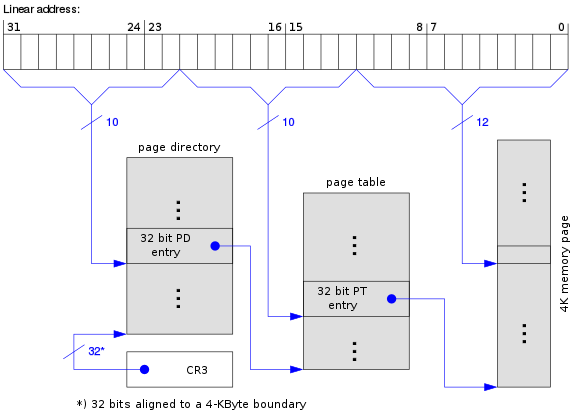
\includegraphics[scale=0.45]{paging-no-pae}
        \caption{Exemple de traduction d'adresse par la MMU sans utiliser la
          technologie PAE}
        \label{fig:paging-no-pae}
      \end{figure}
      \nomenclature{MMU}{Memory Management Unit}

      Ce mécanisme fût introduit en 1995 dans les premiers Pentium Pro, et
      fonctionne de la manière suivante. Considérons une MMU classique
      (figure~\ref{fig:paging-no-pae}) permettant de gérer des adresses de 32
      bits. Celle-ci contient deux niveaux d'indirection, chacun ayant 1024
      entrées de 4 octets. Lors d'une traduction, on utilise les
      MSB\nomenclature{MSB}{Most Significant Bit} comme index dans chacune des
      indirections, puis les LSB\nomenclature{LSB}{Least Significant Bit} pour
      obtenir l'offset.

      Chaque processus a dans son espace virtuel un pointeur vers une adresse
      physique. À cette adresse se trouve le \textit{Page Directory}. Les
      entrées de ce tableau (appelées PDE\nomenclature{PDE}{Page Directory
        Entry} sont indexées par les 10 premiers bits de l'adresse virtuelle que
      l'on veut accéder. Elles sont stockées sur 32 bits, et le \textit{Page
        Directory} contient 1024 entrées ($2^{10} = 1024$). Les PDE contiennent
      le numéro de la page mémoire où est située la \textit{Page Table} du
      processus. Ce numéro est appelé PFN\nomenclature{PFN}{Page Frame
        Number}. Comme le \textit{Page Directory}, la \textit{Page Table} est
      indexée par 10 bits. Elle a donc une profondeur de 1024, et les entrées
      (PTE\nomenclature{PTE}{Page Table Entry}) sont stockées sur 32 bits. Ces
      PTE contiennent le PFN de la page contennant la donnée que l'on cherche à
      accéder. À partir de ce PFN, on peut retrouver l'adresse physique de la
      page correspondante, puis on utilise les 12 bits d'offset restant pour se
      déplacer et obtenir la donnée.

      \begin{paragraph}{Remarque:}
        Le noyau Linux utilise quatre niveaux d'abstraction dans sa version
        actuelle. Néanmoins, ils sont purement logiciels. La MMU continue de
        travailler avec deux niveaux d'indirection comme dans la
        figure~\ref{fig:paging-no-pae}.\\
      \end{paragraph}
      
      L'activation du mode PAE dans la MMU permet de rajouter un troisième
      niveau d'indirection, en diminuant le nombre de MSB utilisés
      précédement. On voit sur la figure~\ref{fig:paging-pae} que les bits 30 et
      31 sont maintenant réservés à une nouvelle table, la
      PDPT\nomenclature{PDPT}{Page Directory Pointer Table} (\textit{Page
        Directory Pointer Table}). Le mode PAE transforme également la taille
      des entrées du \textit{Page Directory} et de la \textit{Page Table} en
      entrées de 64 bits et non plus 32. Pour ce faire, on considére que le
      nombre d'entrées dans ces tables est maintenant de 512, et que chaque
      entrée est la concaténation de deux entrées de 4 octets. On obtient donc
      des \textit{PDE} et des \textit{PTE} sur 8 octets contenant des
      \textit{PFN} sur 64 bits.

      \begin{figure}[ht]
        \centering 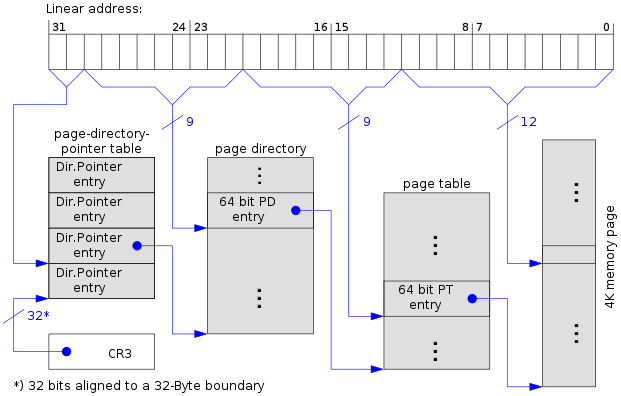
\includegraphics[scale=0.45]{paging-pae}
        \caption{Exemple de traduction d'adresse par la MMU avec la technologie
          PAE}
        \label{fig:paging-pae}
      \end{figure}
      
      Ce mécanisme permet donc à la MMU d'accéder à des adresses sur 64 bits, et
      ainsi de dépasser les 4Go imposés par les espaces d'adressages de 32
      bits. Néanmoins, l'adressage physique est lui restreint à 36 bits, ce qui
      implique une limite à 64Go ($2^{36}$).

      \begin{paragraph}{Remarque:}
        \begin{itemize}
          \item Le mode PAE existe également dans les processeurs
            AMD~\citep{amd2000system}
          \item Microsoft a pour sa part développé
            AWE~\citep{russinovich2012windows}\nomenclature{AWE}{Address
              Windowing Extension}, qui est une
            API\nomenclature{API}{Application Programming Interface} utilisateur
            basée sur PAE. Cette API propose aux développeurs d'applications
            d'exploiter eux aussi plus de 4Go de mémoire.
        \end{itemize}
      \end{paragraph}


    \subsection{Large Physical Address Extension}

    Les processeurs ARM apparus dans les années 90 ont anticipé cette faible
    limite de 64Go et ont proposé leur propre mécanisme, appelé
    LPAE~\citep{arm2012principles,marinas2011linux}\nomenclature{LPAE}{Large
      Physical Address Extension}, pour \textit{Large Physical Address
      Extension}.

    Sur le même principe que PAE, les processeurs proposent un découpage des
    adresses virtuelles en trois niveaux d'indirection, chacun contenant des
    entrées sur 64 bits. Le premier permet d'avoir des pages de 1Go, le second
    de 2Mo, et le dernier de 4Ko.

    L'extension à 40 bits permet de supporter une mémoire de 1To maximum, et non
    plus 64Go comme le proposait PAE. Malgré tout, l'utilisation des processeurs
    32 bits implique d'avoir un certain nombre d'informations stockées dans la
    première portion de 4Go, et notamment:

    \begin{itemize}
      \item le code de boot
      \item un certaine quantité de RAM\nomenclature{RAM}{Random-Access Memory}
        pour le noyau
      \item les registres des périphériques\footnote{Notamment les périphériques
        64 bits qui doivent être adressables par le noyau qui lui est 32 bits.}
      %% \item les régions dynamiquement allouées pour les
      %%   entrées/sorties\footnote{Il n'est pas obligatoire que ces régions
      %%   soient toutes mappées dans les quatre premiers giga.}
    \end{itemize}

    La figure~\ref{fig:arm-0-1024} nous montre comment l'espace mémoire est
    découpé selon les limitations de 32, 36 et 40 bits.

    \begin{figure}[ht]
      \begin{subfigure}[b]{0.37\textwidth}
        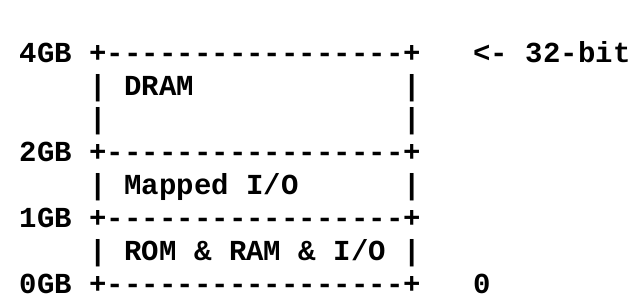
\includegraphics[scale=0.24]{arm-0-4}
        \caption{Découpage $0-4Go$}
        \label{fig:arm-0-4}
      \end{subfigure}
      \begin{subfigure}[b]{0.37\textwidth}
        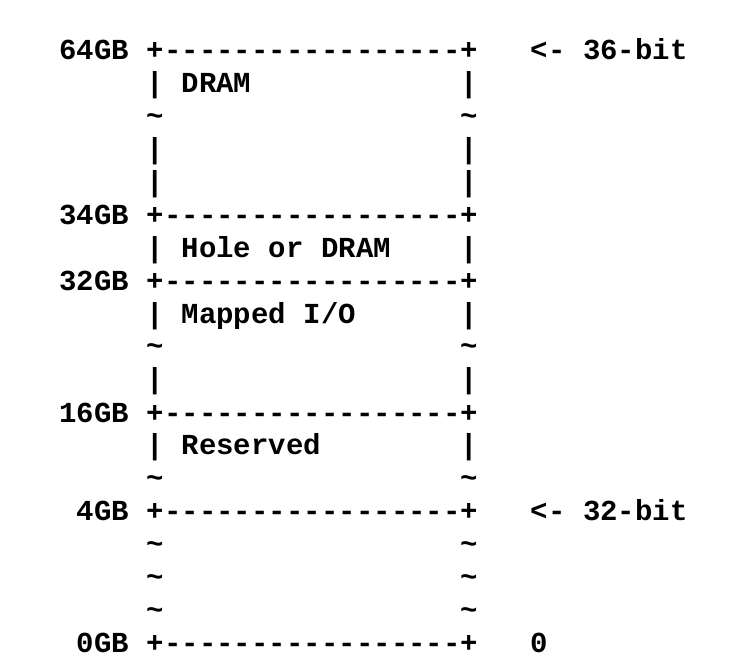
\includegraphics[scale=0.24]{arm-4-64}
        \caption{Découpage $4-64Go$}
        \label{fig:arm-4-64}
      \end{subfigure}
      \begin{subfigure}[b]{0.23\textwidth}
        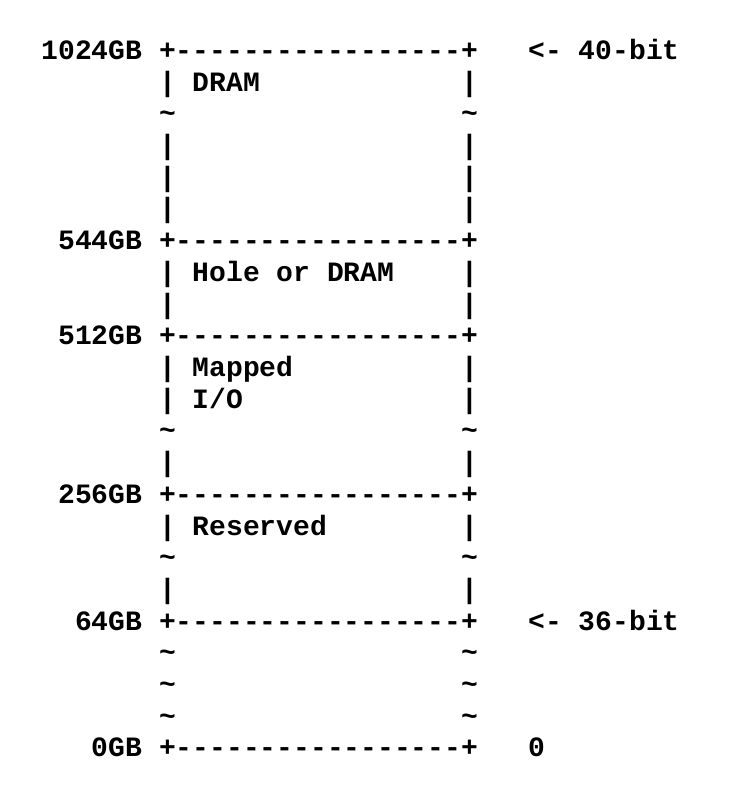
\includegraphics[scale=0.24]{arm-64-1024}
        \caption{Découpage $64-1024Go$}
        \label{fig:arm-64-1024}
      \end{subfigure}
      \caption{Découpage de l'espace mémoire sur un processeur ARMv7 avec le
        mécanisme LPAE~\citep{arm2012principles}.}
      \label{fig:arm-0-1024}
    \end{figure}

    On remarque sur les figures (b) et (c) deux ``trous'' mémoire pour un total
    de 32Go. Ces derniers sont optionnels et peuvent être alloués pour des
    données~\citep{arm2012principles}. On obtient le schéma suivant:

    \begin{itemize}
      \item 512Go de données (extensible à 544Go)
      \item 273Go pour les entrées/sorties
      \item 204Go de réservés
      \item 1Go (le premier) pour la ROM\nomenclature{ROM}{Read-Only Memory}, la
        RAM et les périphériques adressables
    \end{itemize}

    Les processeurs ARM étant des processeurs RISC 32 bits, ils remplissent
    parfaitement les pré-requis nécessaires de l'architecture TSAR. De plus, ils
    sont conçus de manière à avoir une (très) faible consommation électrique, ce
    qui est idéal dans notre cas.

    \begin{paragraph}{Remarque:}
      L'extension LPAE supporte le mode \textit{Hypervisor} des processeurs ARM
      permettant de gérer la para-virtualisation avec des outils comme
      Xen~\cite{barham2003xen}. Bien qu'en dehors du cadre de ce stage, c'est
      une caractéristique très intéressante pour le projet
      TSUNAMY~\cite{tsunamy2013web}\nomenclature{TSUNAMY}{TODO} dans lequel
      l'équipe ALSOC\nomenclature{ALSOC}{Architecture et Logiciels pour Systèmes
        On Chip} est engagée.
    \end{paragraph}


    \subsection{Les noyaux monolithiques classiques (UNIX et NT)}
    \nomenclature{UNIX}{Uniplexed Information and Computing Service}

      Les noyaux monolithiques ont exploité cette avancée matérielle en
      supportant de manière logicielle le mode PAE. Pourtant, il existe des
      contraintes très fortes lorsque l'on utilise ce mode d'adressage. Dans un
      premier temps, on ne supporte que 64Go de RAM. Bien que conséquente en
      1998, cette valeur nous paraît aujourd'hui trop petite, compte tenu de la
      puissance à venir des machines de calcul.  Dans un second temps, cette
      amélioration apporte un problème logiciel qui reste non résolu à ce jour:
      la gestion des descripteurs de page.\\

      La mémoire est découpée de manière abstraite en pages. Ces pages peuvent
      être de grande taille (2Mo ou 4Mo selon les systèmes), ou de petite taille
      (4Ko). Pour adresser la mémoire, le noyau doit construire cette
      abstraction via les descripteurs de pages, puis toutes les opérations en
      mémoire physique passeront par ces descripteurs. Pour connaître en
      permanence l'état global de la mémoire ou l'état d'une page en
      particulier, le noyau doit décrire entièrement l'espace
      adressable~\citep{cranor1999uvm, gorman2004understanding,
        russinovich2012windows, dillon2000design, steldt2009memory,
        steldtXXXXopenbsd}.

      Cette opération est effectuée au boot de la machine. Lorsque l’on dispose
      d’une grosse quantité de mémoire, l'espace physique occupé par ces
      descripteurs est conséquent. Sous Linux, un descripteur de pages fait 44
      octets. Pour décrire 1Go de mémoire, Linux a donc besoin de
      11Mo\footnote{$0,044*1.10^6/4 = 11.10^3Ko = 11Mo$} de structure de données
      représentant ces pages. Si l'on augmente à 16Go, Linux a maintenant besoin
      de 176Mo pour décrire la mémoire. En sachant que le noyau ne s'accorde que
      1Go de mémoire, et qu'il a besoin de ce giga-octet pour de multiple
      opérations, on ne peut pousser trop loin l'utilisation de la technologie
      PAE sans risquer de prendre trop de place en mémoire noyau et de voir des
      chutes de performances, voire un crash total\footnote{Le noyau ne peut pas
        swapper ses propres pages sans risquer de perdre des informations
        vitales. S'il n'a plus de place, sa seule possibilité est de lancer un
        \texttt{panic} et de s'arrêter.}. Cette valeur, bien qu’élevée, est
      supérieure dans le noyau ALMOS, car les structures représentant les pages
      sont plus volumineuses en mémoire que celle de Linux ou *BSD. En effet, un
      descripteur de page fait 56 octets. Le noyau a donc besoin de 14Go pour
      décrire les 1To de mémoire offerts par TSAR. Le
      tableau~\ref{tab:pages-desc} montre un comparatif de la place occupée par
      ces descripteurs dans Linux et ALMOS.

      %% Change space between rows and columns
      \FloatBarrier
      \setlength{\tabcolsep}{10pt}
      \renewcommand{\arraystretch}{1.5}
      \begin{table}[htp]
        \centering
        \begin{tabular}{cc|c|c|c}
          \cline{3-4} & & \multicolumn{2}{c|}{Noyau} & \\ \cline{3-4} & & Linux
          & ALMOS & \\ \cline{1-4} \multicolumn{1}{|c|}{\multirow{3}{*}
            {\begin{tabular}[c]{@{}c@{}}M\\ e\\ m\end{tabular}}} & 1Go & 11Mo &
          57Mo & \\ \cline{2-4} \multicolumn{1}{|c|}{} & 16Go & 176Mo & 224Mo &
          \\ \cline{2-4} \multicolumn{1}{|c|}{} & 1To & 11Go & 14Go &
          \\ \cline{1-4}
        \end{tabular}
        \caption{Place occupée par les descripteurs de pages dans les noyaux
          Linux et ALMOS. Afin de simplifier les résultats, les calculs ont été
          fait avec des puissances de 10 et non de 2 ($1Go = 10^{3}$ et non pas
          $2^{10}$)}
        \label{tab:pages-desc}
      \end{table}
      %% Restore default parameters
      \setlength{\tabcolsep}{6pt}
      \renewcommand{\arraystretch}{1.0}
      \FloatBarrier

    \subsection{Conclusion}

      Les industriels ont apporté des solutions à ce problème qu'ils considèrent
      comme important. Les mécanismes de PAE ou de LPAE sont un bon exemple de
      solutions efficaces et fonctionnelles, bien que PAE soit limité à
      64Go. Néanmoins, les noyaux classiques, et notamment Linux, ont choisi de
      ne pas supporter entièrement ces mécanismes et de ne pas traiter ce
      problème en considérant que ce n'en est pas un. En effet, les développeurs
      n'ont pas vu les avantages à conserver des architectures 32 bits, et
      invitent à passer sur des architecture 64
      bits~\citep{gorman2004understanding} pour la gestion de grosses quantité
      de mémoire. Nous pensons que les architectures 64 bits ne sont pas une
      voie optimale pour les architectures massivement multi-c\oe urs. De plus,
      la gestion de grands espaces d'adressage mérite d'être traitée pour
      apporter une solution logicielle efficace aux technologies matérielles
      proposées par Intel ou ARM sur leurs processeurs.

  
  \section{Passage à l’échelle des noyaux}
  \label{sec:scalability}

    TSAR est une architecture massivement multi-c\oe urs
    cc-NUMA\nomenclature{cc-NUMA}{Cache-Coherent Non-Uniform Memory Access} à
    mémoire partagée. Ainsi, en plus de disposer d'une grande mémoire, elle est
    composée d'un grands nombre de c\oe urs, répartis en clusters. Ce découpage
    implique que les accès mémoire se font à deux vitesses: si un processeur
    accède à la mémoire de son cluster, la réponse sera plus rapide que s'il
    veut accéder à la mémoire du cluster voisin. La localité de ces accès
    mémoire est au c\oe ur des problématiques des architectures NUMA. %%Nous
    %% allons donc nous intéresser dans cette seconde partie aux différents
    %% travaux qui adressent cette problématique.


    \subsection{Scalabilité du noyau Linux}

      Il paraît évident dans un premier temps de vouloir adapter le noyau Linux
      à des architectures massivement multi-c\oe urs. En effet, changer de noyau
      alors que ce dernier s’est imposé partout est un pari très risqué et très
      difficile. À cet effet,~\citet{boyd2010analysis} ont étudié la scalabilité
      de Linux sur une machine 48 c\oe urs en utilisant le benchmark
      MOSBENCH\nomenclature{MOSBENCH}{Multicore Operating Systems
        Benchmark}. Ils ont pu tirer plusieurs conclusions de cette étude.
      Premièrement, il existe trois types de problèmes liés au passage à
      l’échelle :
      \begin{itemize}
        \item l’implémentation du noyau
        \item l’implémentation de l’application utilisateur
        \item la façon dont l’application utilise les services du noyau
      \end{itemize}
      Grâce à cela,~\citeauthor{boyd2010analysis} sont parvenus à résoudre les
      problèmes liés aux applications de MOSBENCH, et ce en utilisant des
      techniques basiques de programmation parallèle. De plus, la grande
      majorité de leurs contributions sur le noyau ne sont que de petits
      changements très localisés. Seule la gestion des compteurs de références
      pour le \textit{garbage collector} a été grandement
      modifiée\footnote{Voir~\citep{boyd2010analysis} et les \textit{sloppy
          counters}.}.

      Ainsi, ils sont parvenus à identifier les problèmes du noyau, comme par
      exemple la gestion du cache des \texttt{dentry} ou les goulots formés par
      les sytèmes de fichiers montés (\texttt{vsfmount}), et à les résoudre pour
      obtenir des performances acceptables.

      Néanmoins, nous pouvons aujourd’hui adresser trois critiques à ces travaux
      :
      \begin{itemize}
        \item le noyau utilisé est ancien (2.6.35-rc5, 12 Juillet 2010). Les
          mécanismes de préemption venaient d’être ajoutés et n’étaient pas
          aussi performants qu'aujourd'hui
        \item la machine considérée est composée de seulement 48 c\oe urs, ce qui
          est peu par rapport à la puissance des machines actuelles
        \item leur propre conclusion indique qu’il ne faut pas changer le design
          des sytèmes d’exploitation `` pour l’instant''\\
      \end{itemize}
      Nous pensons qu’à présent, il est nécessaire de revoir cette organisation.

      
    \subsection{Popcorn Linux}

      Le projet Popcorn Linux~\citep{barbalacepopcorn} part du même constat
      évoqué précédement, mais en essayant tout de même de conserver Linux comme
      base de travail. Avec un noyau plus récent que l'étude précédente (3.2),
      ils ont en partie adopté les principes du multi-noyau mais en ont rejeté
      certains.\footnote{Notamment l'hétérogénéité des
        architectures~\citep{schupbach2008embracing} qui n'est pas du tout
        abordée dans ce projet.}\\

      Popcorn Linux permet de lancer plusieurs noyaux Linux en même temps sur la
      même machine. Le matériel est attribué de manière logicielle entre les
      différentes instances du noyau, et ces dernières communiquent uniquement
      par passage de messages~\citep{shelton2013popcorn}. Afin de garantir à
      l’utilisateur l’illusion d’un seul système en cours d'exécution, les
      noyaux utilisent ces messages pour construire `` l’image disque unique''
      (\textit{Single System Image}, figure~\ref{fig:popcorn-layers}). C'est
      cette abstraction qui est proposée à l'utilisateur, lui masquant
      entièrement l'aspect multi-noyau du système.

      \begin{figure}[ht]
        \centering
        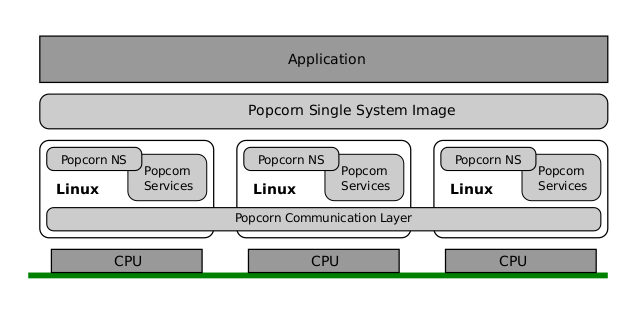
\includegraphics[scale=0.44]{popcorn-layers}
        \caption{Architecture logicielle du noyau Popcorn Linux. La couche de
          communication assure à l'utilisateur l'illusion d'un unique
          noyau~\citep{barbalacepopcorn}.}
        \label{fig:popcorn-layers}
      \end{figure}

      Le partitionnement des ressources est fait selon la configuration donnée
      au boot du noyau, mais il est également possible de redéfinir
      l'attribution des ressources pendant l'exécution d'un noyau. Le premier
      noyau qui est lancé, appelé `` noyau maître'', lance un processus de
      reconnaissance du matériel. Ensuite, on précise aux noyaux secondaires,
      via des paramètres au boot, les ressources dont ils peuvent disposer. Une
      fois les noyaux lancés, ils ne partagent aucune données, exception faite
      de la table contenant les adresses d’écriture des buffers des autres
      noyaux, utilisée pour le passage de messages (voir
      figure~\ref{fig:popcorn-buf}). Ces buffers sont de type ``
      MWSR''\nomenclature{MWSR}{Multi Writer Single Reader} et utilisent un
      système de ticket pour les écritures. Les lectures utilisent un mélange de
      deux techniques:\benumline \item le lecteur viendra consulter de manière
      régulière le contenu de son buffer (\textit{polling}) ou \item il ira lire
      le buffer sur réception d’une IPI\nomenclature{IPI}{Inter-Processor
        Interruption} du c\oe ur ayant initié l’écriture\eenumline.

      \begin{figure}[ht]
        \centering
        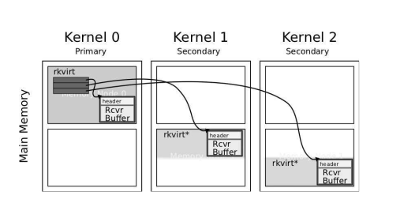
\includegraphics[scale=0.7]{popcorn-buffers}
        \caption{Les différents noyaux doivent impérativement mapper le tableau
          \texttt{rkvirt} dans leur espace d'adressage pour pouvoir communiquer
          avec les autres. L'adresse de ce tableau est fixe et connue de tous.
          Lorsqu'un noyau secondaire est lancé, il ajoute l'adresse de son
          buffer dans ce tableau~\citep{barbalacepopcorn}.}
        \label{fig:popcorn-buf}
      \end{figure}

      Ces communications permettent de donner l’illusion qu’il n’y a qu’un seul
      noyau en cours d’exécution, mais aussi de pouvoir migrer des tâches entre
      les différentes instances de noyaux de manière
      transparente~\citep{katz2013popcorn}.\\

      Les tests de performances effectués sur Popcorn Linux se sont montrés
      décevants. D'une part parce que la machine considérée ne contient que 48
      c\oe urs et 64Go de mémoire, et d'autre part parce que les résultats des
      tests n'ont pas montrés d'améliorations significatives des
      performances. Au contraire, il apparaît que Popcorn Linux est
      majoritairement mois efficace que Linux, sauf dans quelques
      cas\footnote{L'utilisation de gmake pour la compilation noyau par
        exemple.}. Ce résultat est à relativiser, car une seule suite de
      benchmark a été utilisée ici. En revanche, ce projet ne s'attaque pas à la
      problématique des très grands espaces d'adressages physiques sur des
      architectures 32 bits.


    \subsection{Barrelfish}
      
      L’ETH Zurich, en collaboration avec Microsoft Research, a engagé des
      travaux de recherche dans le domaine des architectures du futur en
      2008. Leurs équipes sont parvenues à établir un nouveau modèle de
      construction des systèmes d’exploitation : le
      multi-noyau~\citep{baumann2009multikernel}. Ce paradigme part de plusieurs
      postulats:
      \begin{itemize}
        \item les architectures du futur seront très
          hétérogènes~\citep{schupbach2008embracing}
        \item les noyaux actuels ne profitent pas de l’hétérogénéité offerte par
          le matériel et au contraire essayent de la masquer au maximum
        \item les machines sont construites comme des systèmes distribués,
          pourquoi ne pas appliquer le même modèle aux systèmes
          d’exploitation~\citep{baumann2009your}.\\
      \end{itemize}

      Selon l’approche multi-noyau (voir figure~\ref{fig:barrelfish}),
      l'environnement d’exécution des applications est une collection de n\oe
      uds où chaque n\oe ud est constitué d’un c\oe ur exécutant un système
      d'exploitation à base d’un micro-noyau : Barrelfish. Les communications
      entre les différents systèmes se font par passage de messages. Le système
      utilise une variante des Remote Procedure Calls au niveau utilisateur
      (URPC). Chaque noyau dispose d’un serveur système en mode utilisateur
      appelé Monitor. L’ensemble des moniteurs coordonne collectivement l’accès
      à l’état global du système et maintient la cohérence des structures de
      données répliquées par c\oe ur (les tables d’allocation mémoire et les
      mappings des espaces d’adressages virtuels).\\

      \begin{figure}[ht]
        \centering 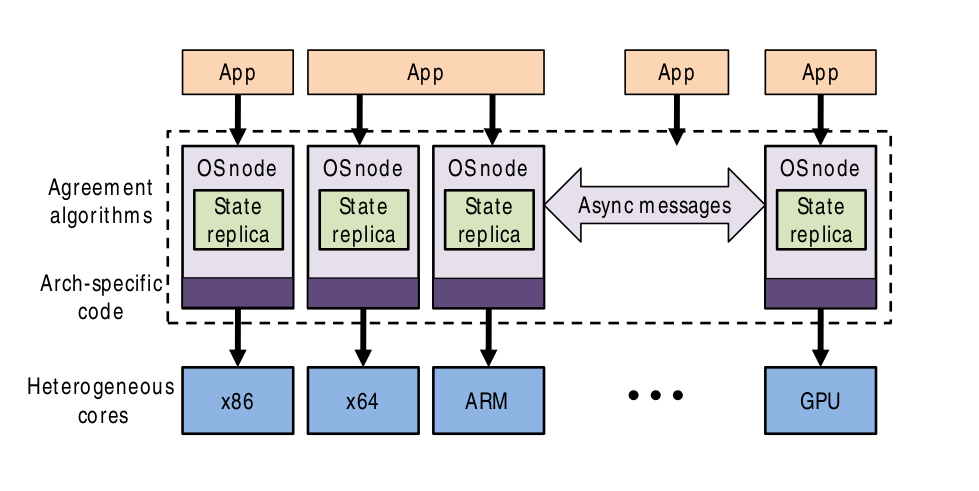
\includegraphics[scale=0.3]{barrelfish}
        \caption{L'architecture multi-noyau de
          Barrelfish~\citep{baumann2009multikernel}.}
        \label{fig:barrelfish}
      \end{figure}

      \citeauthor{baumann2009multikernel} ont ``stressé'' Barrelfish avec
      différents benchmarks. Les résultats sont montrés par la
      figure~\ref{fig:barrelfish-bench}. On voit que Barrelfish comme Popcorn
      Linux ne montre pas d'augmentation de performances
      significative. Néanmoins, ce résultat est à relativiser. Il démontre que
      Barrelfish, qui est un noyau jeune et construit \textit{from scratch},
      peut obtenir des performances similaires voire supérieures à Linux.

      \begin{figure}[ht]
        \centering
        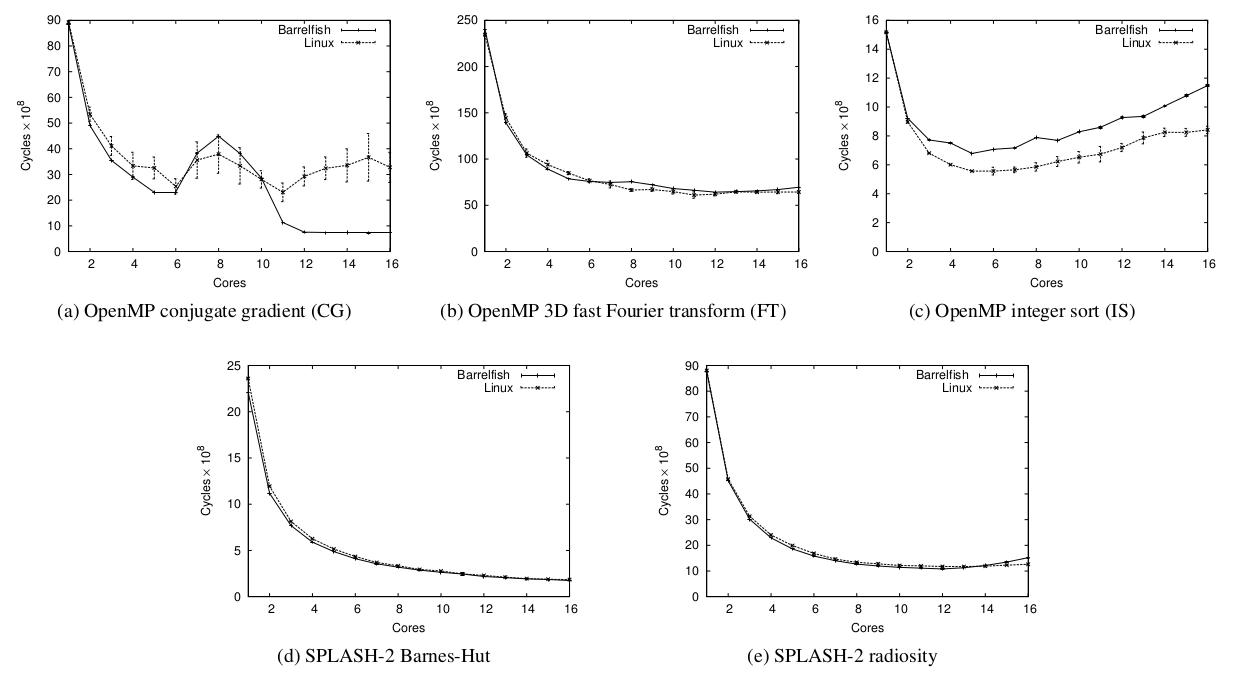
\includegraphics[scale=0.33]{barrelfish-bench}
        \caption{Résultats de benchmark \textit{compute-band} sur une machine
          AMD à 16 c\oe urs~\citep{baumann2009multikernel}.}
        \label{fig:barrelfish-bench}
      \end{figure}

    \subsection{Autres travaux}
    \label{subsec:others}
    
      \begin{paragraph}{Hurricane:}

        Parmi les premiers travaux sur la scalabilité des systèmes
        d’exploitation se trouve la thèse d’Unrau. Ce dernier a formulé trois
        grands principes pour une conception scalable d’un système
        d’exploitation qui sont : \benumline \item préserver le
        parallélisme \item préserver la localité et \item borner le surcoût des
        services\eenumline. \citet{unrau1995hierarchical} ont proposé le système
        d’exploitation Hurricane à base de micro-noyau avec une approche de
        conception nommée Hierarchical Clustering.\\

        Selon cette approche, le système d’exploitation est vu en tant qu’une
        collection de clusters. Un cluster est un système d’exploitation complet
        à base de micro-noyau prenant en charge un faible nombre de
        processeurs. Il existe donc autant d’instances du système d’exploitation
        que de clusters. Les serveurs systèmes (en mode utilisateur) de chaque
        cluster coopèrent entre eux pour donner aux applications une vision
        globale d’un seul système d’exploitation. Étant donné que chaque cluster
        propose l’ensemble des services système via des serveurs dédiés,
        l’existence de plusieurs clusters constitue une réplication des mêmes
        services et augmente la disponibilité du système. La dimension en nombre
        de processeurs d’un cluster est un compromis entre le coût des accès
        intra et inter-clusters.\\

        Un envoi de message est réalisé par l’interruption du cluster cible
        pour\benumline \item l’allocation d’un tampon mémoire pour réceptionner
        le message \item copier le message et les informations de contrôle
        depuis le processus émetteur du cluster source et \item attacher le
        tampon à la file d’attente du processus destinataire du
        message\eenumline. Quand un client demande un service, il change son
        espace d’adressage pour celui du serveur et invoque un thread de
        traitement associé à sa requête avant de retrouver son espace
        d’adressage initial.

      \end{paragraph}
      
      \begin{paragraph}{Corey:}

        Avant leurs travaux sur Linux,~\citet{boyd2008corey}. ont proposé le
        système d’exploitation Corey. Dans ce dernier, la gestion du partage des
        ressources est laissée aux applications utilisateurs. Pour cela, trois
        abstractions ont été proposées: \benumline \item \textit{Adresse Range}
        qui permet au programmeur d’une application de décider par c\oe ur
        quelle partie de l’espace d’adressage est privée et laquelle est
        partagée \item \textit{Kernel Core} qui permet au programmeur d’une
        application d’affecter un service noyau à un c\oe ur en particulier
        (piloter une carte réseau par exemple) et \item \textit{Shares} qui
        permet au programmeur d’une application de contrôler le degré de partage
        de certaines tables de correspondances au niveau noyau (par exemple la
        table de descripteurs des fichiers ouverts par le
        processus)\eenumline.\\

        En donnant le contrôle aux programmeurs des applications utilisateur,
        Corey permet en effet de personnaliser le comportement du noyau selon
        les besoins et les spécificités d’une application. Les inconvénients
        majeurs de cette approche sont: \benumline \item de lier fortement
        l’application au système qui l’exécute, ce qui élimine complètement ou
        partiellement la portabilité des applications et complique sérieusement
        la réutilisation du code existant \item d'augmenter la complexité de
        programmation et nécessiter d’avantage d’efforts de la part des
        programmeurs d’applications (gestion explicite des régions virtuelles,
        placement et partage des structures de données noyau, etc.) et \item de
        générer des conflits dans le cas d'exécutions simultanées
        d'applications\eenumline.

      \end{paragraph}

      \begin{paragraph}{FoS:}
      \nomenclature{FoS}{Factored Operating System}

        Des travaux de recherches similaires visant à repenser le système
        d’exploitation sous forme d’une collection de systèmes communicants par
        passage de messages ont été menés par~\citet{wentzlaff2009factored} avec
        FoS. L’objectif de ce projet est de concevoir un système à la fois pour
        processeur massivement multi-c\oe urs et pour les infrastructures de
        Cloud Computing. Comme dans le cas de Barrelfish, chaque c\oe ur exécute
        une instance de système, basé sur un micro-noyau.
        %% comme il est illustré par la figure~\ref{fig:fos}.

        %% \begin{figure}[ht]
        %%   \centering
        %%   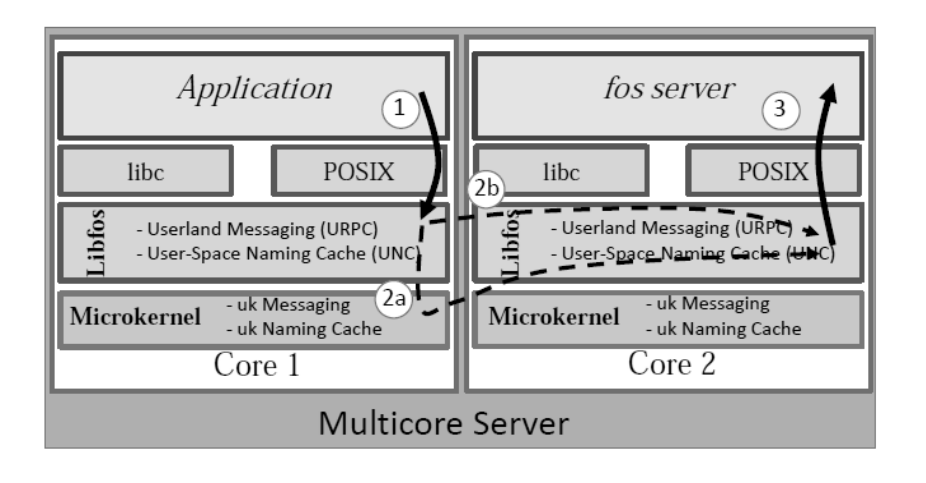
\includegraphics[scale=0.3]{fos}
        %%   \caption{Apercu de la structure interne du noyau FoS et du schéma de
        %%     communication.~\citep{wentzlaff2010operating}}
        %%   \label{fig:fos}
        %% \end{figure}

        FoS permet de spécifier aux différents noyaux en cours d'exécution
        quelles sont les ressources matérielles dont il peut disposer. En se
        fondant sur le partitionnement spatial des ressources de calcul,
        certaines instances exécutent alors des serveurs systèmes, tandis que
        d’autres exécutent des applications. À la différence de Barrelfish, FoS
        se focalise sur la parallélisation des services systèmes pour faire face
        à une demande massive et variable de services.\\

        Concernant les évaluations expérimentales, les principales publications
        autour du projet FoS~\citep{wentzlaff2009factored,
          wentzlaff2010operating} n’incluent pas d'évaluation de scalabilité en
        utilisant des benchmarks.

      \end{paragraph}
      
    \subsection{Influences}

      Bien que ces travaux n'apportent pas de réponse claire et définitive à
      notre problématique, ils nous permettent de mieux comprendre les choix qui
      ont été fait dans le noyau ALMOS. Premièrement, les travaux sur Barrelfish
      ont apporté un nouveau modèle architectural pour la conception d'un
      noyau. Ce modèle semble cohérent et répond aux besoins des architectures
      du futurs. C'est donc le modèle qui a été retenu par ALMOS\footnote{Nous
        verrons plus en détail en section~\ref{sec:almos} le choix du
        multi-noyau.}. Néanmoins, Barrelfish ne respecte pas du tout les
      standards POSIX\nomenclature{POSIX}{Portable Operating System
        Interface}. C'est un choix très fort qui a été fait pour ce projet, et
      qui nous apparaît comme infondé.

      Les travaux sur Popcorn Linux, basé lui aussi sur le modèle du
      multi-noyau, ont permis de montrer que le noyau Linux, qui se veut être
      \textit{POSIX compliant}, peut être adapté à des architectures massivement
      parallèles, tout en respectant les normes. Le projet ALMOS, tout comme
      Popcorn Linux, a fait le choix d'avoir un système respectant au maximum
      les standards de conception des noyaux déjà existants.

      Enfin, les notions de hiérarchisation et de clusters, initalement
      apportées par~\citet{unrau1995hierarchical} et poussées à l'extrême dans
      le noyau Barrelfish\footnote{Un cluster est composé d'un seul processeur
        et non pas d'un ensemble.}, sont une partie intégrante de l'architecture
      TSAR et du noyau ALMOS.\\

      Pourtant, ces recherches ne répondent pas à un des problèmes majeurs de
      l'architecture TSAR. En partant du principe que les processeurs
      d'aujourd'hui manipulent des informations sur 64 bits, les problèmes de
      gestion d'une grande quantité de mémoire ont été effacés.


  \section{Partage et maintien de cohérence de structures noyaux}
  \label{sec:consistency}

    Le modèle du multi-noyau proposé par~\citeauthor{baumann2009multikernel}
    apporte son lot de solutions quant à la gestion des architectures du
    futur. Néanmoins, il subsiste un problème inhérent au multi-noyau: la
    cohérence des données. En effet, l'un des trois principes fondateurs de ce
    modèle est: ``voyez les états comme répliqués et non
    partagés''\footnote{\textit{``View state as replicated instead of
        shared''}}~\citep{baumann2009multikernel}. Pourtant, il faut être
    capable de fournir à l'utilisateur une vision unique du système
    d'exploitation tout en maintenant le partage de ces données.

    Nous nous intéressons ici aux espaces mémoire, aux descripteurs de fichiers
    et aux signaux. Ces deux dernier points représentent les données critiques
    qui nous intéresse dans le cadre de la création distante ou de la migration
    de processus/threads.

    \subsection{Corey}
    \label{subsec:corey}

      Comme nous l'avons vu précédemment, Corey permet de manipuler très
      précisément le partage des données des processus, et notamment celui des
      descripteurs de fichiers.~\citeauthor{boyd2008corey} ont identifié, via un
      simple microbenchmark, que ces derniers posent problème au fur et à mesure
      que l'on augmente le nombre de c\oe urs. L'expérience est la suivante:
      on initialise un certain nombre de threads pour un processus. Chaque
      thread crée un descripteur de fichier, le clone via la fonction
      \texttt{dup()}, puis le ferme avec \texttt{close()}. L'expérience montre
      (figure~\ref{fig:fd-problem}) que plus on augmente le nombre de c\oe urs
      disponibles (et donc la répartition des threads), plus le nombre
      d'opérations par unité de temps diminue.

      \begin{figure}[ht]
        \centering
        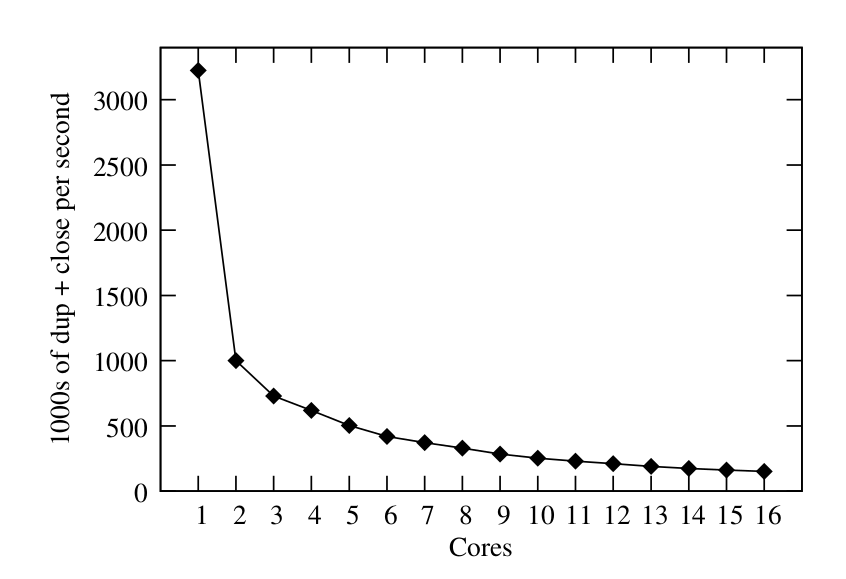
\includegraphics[scale=0.3]{fd-problem}
        \caption{Débit des opérations \texttt{dup()} et \texttt{close()} en
          fonction du nombre de c\oe urs~\citep{boyd2008corey}.}
        \label{fig:fd-problem}
      \end{figure}

      Cela est dû à la norme POSIX, qui spécifie que toute opération d'un thread
      sur un fichier soit visible par les autres threads du même processus. Les
      accès à la table des descripteurs de fichiers se faisant de manière
      atomique, celle-ci est un goulot d'étranglement pour le système.\\

      Pour répondre à cela,~\citeauthor{boyd2008corey} ont poussés le contrôle
      du partage jusqu'aux descripteurs de fichiers. Ainsi, lorsqu'un thread
      ouvre un fichier, il dispose d'un mode permettant d'indiquer au noyau si
      le fichier en question sera partagé. Par défaut il ne l'est pas, ce qui
      implique au programmeur de devoir définir explicitement le partage.

      Ce mécanisme permet de gérer localement les fichiers que le thread
      manipule. Si au cours de l'exécution le fichier doit être partagé, le
      thread change le mode en \texttt{SHARED}, accède de manière atomique à la
      table des descripteurs de fichiers du processus, et ajoute son
      descripteur. Celà permet de réduire significativement la contention sur
      cette structure (figure~\ref{fig:fd-solved-1}), qui se matérialise
      également par le nombre de miss dans le cache L3
      (figure~\ref{fig:fd-solved-2}).

      %% FIXME: figures alignement
      \begin{figure}[ht]
        \begin{subfigure}[b]{0.5\textwidth}
          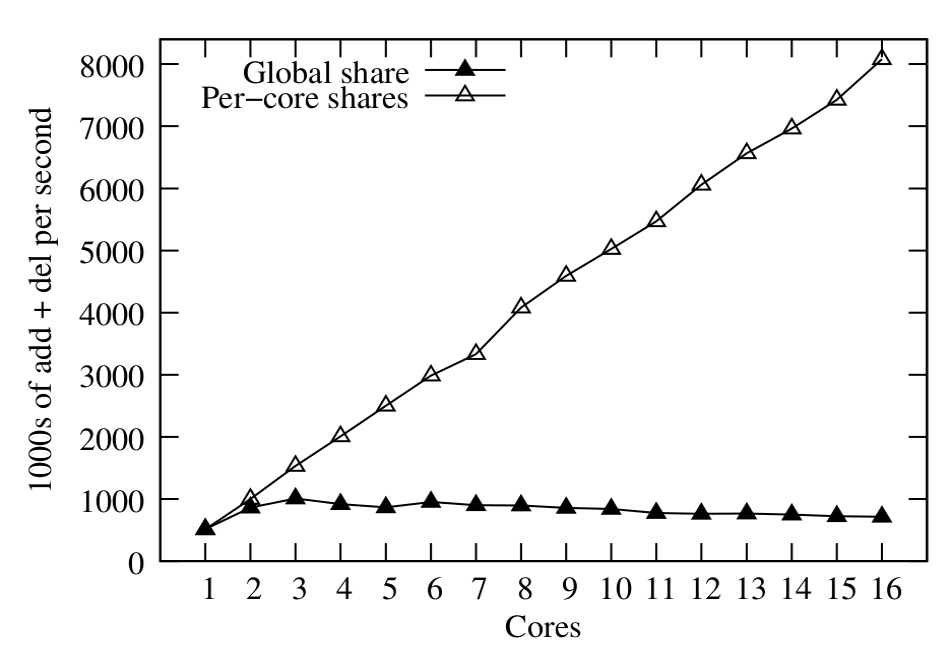
\includegraphics[width=200px]{fd-solved-1}
          \caption{Débit des opérations \texttt{dup} et \texttt{close} en
            fonction du nombre de c\oe urs.}
          \label{fig:fd-solved-1}
        \end{subfigure}
        \begin{subfigure}[b]{0.5\textwidth}
          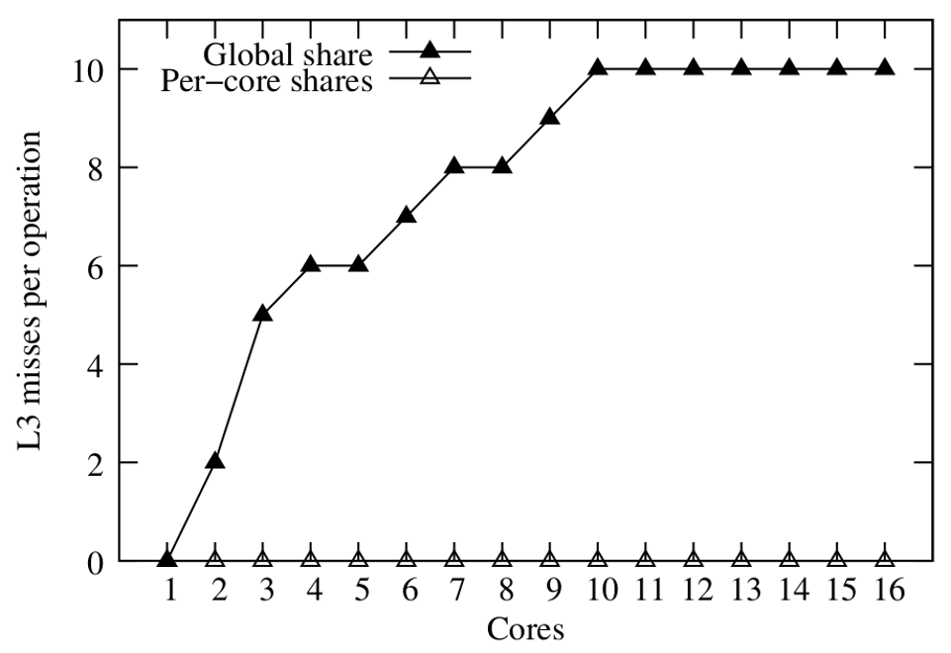
\includegraphics[width=211px]{fd-solved-2}
          \caption{Nombre de miss dans le cache L3.}
          \label{fig:fd-solved-2}
        \end{subfigure}
        \caption{Résultats d'expériences après modification du partage des
          descripteurs de fichiers~\citep{boyd2008corey}.}
      \end{figure}
      \FloatBarrier


    \subsection{Hare}

      Hare~\citep{gruenwald2014providing} est une bibliothèque s'exécutant au
      dessus de Linux en mode multi-noyau. Son but est de fournir un système de
      fichier scalable et cohérent sans utiliser de mécanismes matériels,
      considérés eux comme non scalables. Hare apporte différentes solutions à
      plusieurs niveaux, et notamment concernant la distribution du systeme de
      fichiers et la migration de processus. C'est à ce jour la solution la plus
      complète que nous avons trouvé.\\

      Hare propose de distribuer la gestion des fichiers en utilisant le
      mécanisme client/serveur. Le système de fichiers est géré de manière
      distribuée par des serveurs qui sont eux aussi distribués. Certains noyaux
      ne possèdent pas de serveur. Lors d'un \texttt{open()} se faisant sur un
      noyau n'ayant pas de serveur, le client doit dans un premier temp résoudre
      le nom de celui qu'il doit contacter. Pour cela, la fonction suivante est
      utilisée:
      \begin{center}
        \texttt{hash(dir, name) \% NSERVERS = server\_id}
      \end{center}
      où \textit{dir} représente le chemin vers le fichier désiré, \textit{name}
      le nom de ce fichier, et \texttt{NSERVERS} le nombre de serveurs de
      fichiers présent dans le système\footnote{Ce nombre est fixé au démarrage
        du noyau. Néanmoins, l'auteur précise qu'il travaille à la dynamicité de
        ce paramètre à des fins de performances.}. Une fois que l'identifiant du
      serveur est connu, la demande est effectuée par passage de messages.

      \begin{figure}[ht]
        \centering
        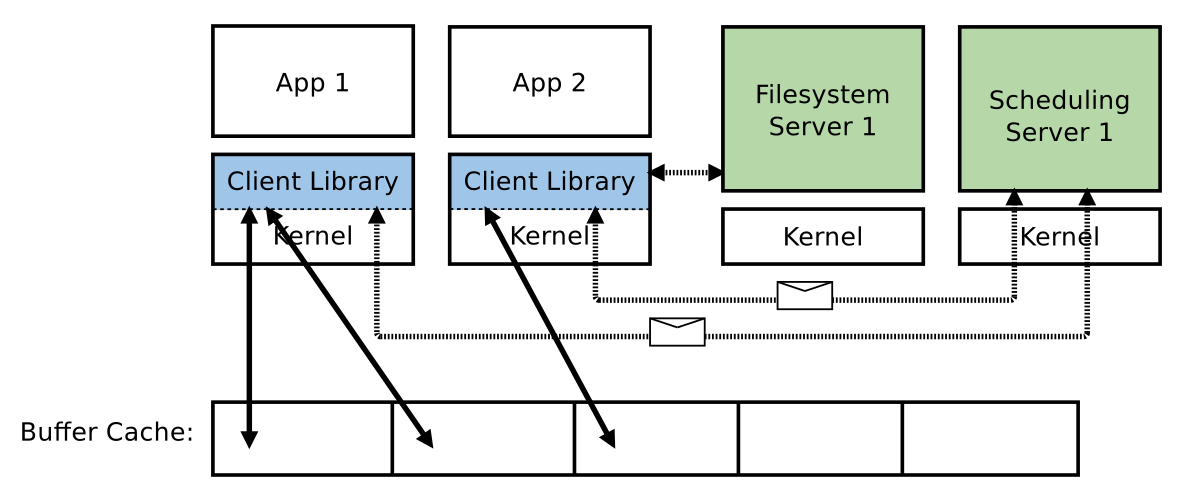
\includegraphics[scale=0.25]{hare-design}
        \caption{Fonctionnement de Hare. Certains noyaux possèdent un serveur de
          fichiers et d'autres non. La communication se fait par passage de
          messages. Les écritures se font dans le buffer-cache qui est
          partagé~\citep{gruenwald2014providing}.}
        \label{fig:hare-design}
      \end{figure}

      Pour gérer le partage de fichiers, Hare utilise un mécanisme nommé
      \textit{Hybrid File Descriptor Tracking} (figure~\ref{fig:hare-fd}). Le
      principe est le suivant:
      \begin{itemize}
        \item les serveurs maintiennent une table des compteurs de références
          sur les inodes qu'ils gèrent
        \item lorsqu'un thread accède à un fichier, ce compteur est incrémenté.
        \item si celui-ci est inférieur ou égal à 1 (\textit{i.e,} le thread est
          le seul à accéder au fichier), le descripteur de fichier que lui
          renvoi le serveur contient le champ \texttt{offset} et sa valeur.
        \item dans le cas où plusieurs threads ont ouvert le même fichier, alors
          la valeur du champ \texttt{offset} est gérée côté du serveur, et
          toutes les opérations sur le fichier devront se faire par passage de
          messages.
      \end{itemize}
      \begin{figure}[ht]
        \centering
        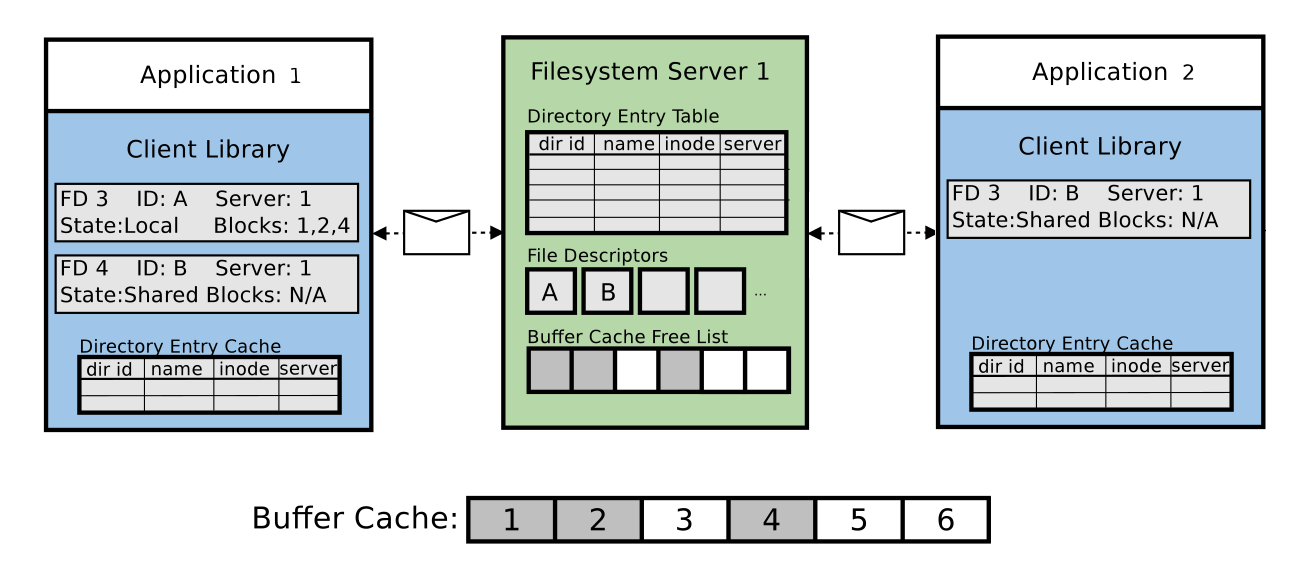
\includegraphics[scale=0.28]{hare-fd-2}
        \caption{Mécanisme de partage des descripteurs de fichiers. Le
          \textit{file desciptor} 3 correspond à un fichier local de
          l'application 1, tandis que le \textit{file descriptor} 4 est partagé
          par les deux applications~\citep{gruenwald2014providing}.}
        \label{fig:hare-fd}
      \end{figure}

      Selon l'auteur, cette solution n'est pas une réponse définitive au
      problème des descripeurs de fichiers. En effet, le serveur représente un
      goulot d'étranglement si de nombreux threads ouvrent le même
      fichier. Néanmoins, elle reste efficace comme en témoigne les résultats de
      la figure~\ref{fig:hare-res}. Enfin, pour des raisons de performances, les
      applications où les threads se partagent un/des fichier(s) ne sont pas
      nombreuses.\\

      \begin{figure}[ht]
        \begin{subfigure}[b]{0.5\textwidth}
          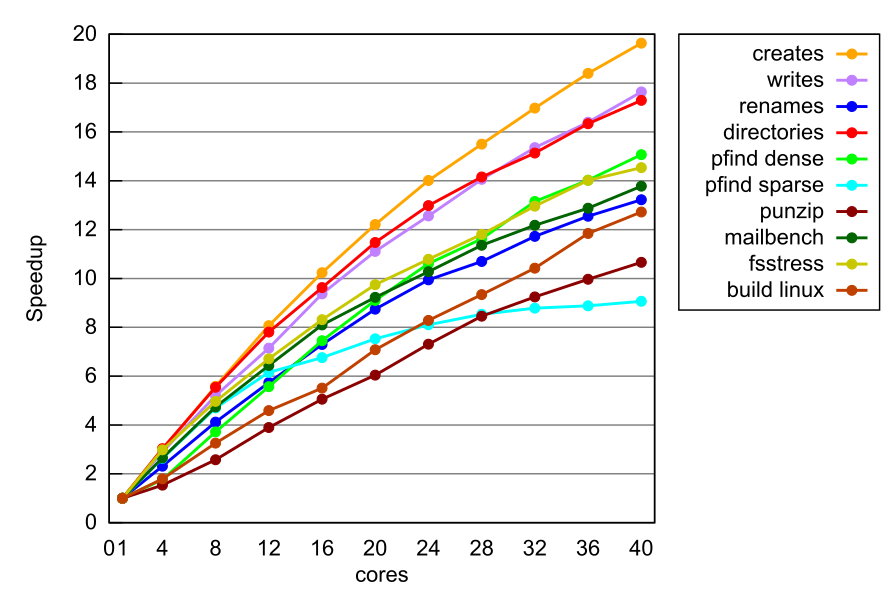
\includegraphics[scale=0.25]{hare-speedup}
          \caption{Accélération en fonction du nombre de c\oe urs}
        \end{subfigure}
        \begin{subfigure}[b]{0.5\textwidth}
          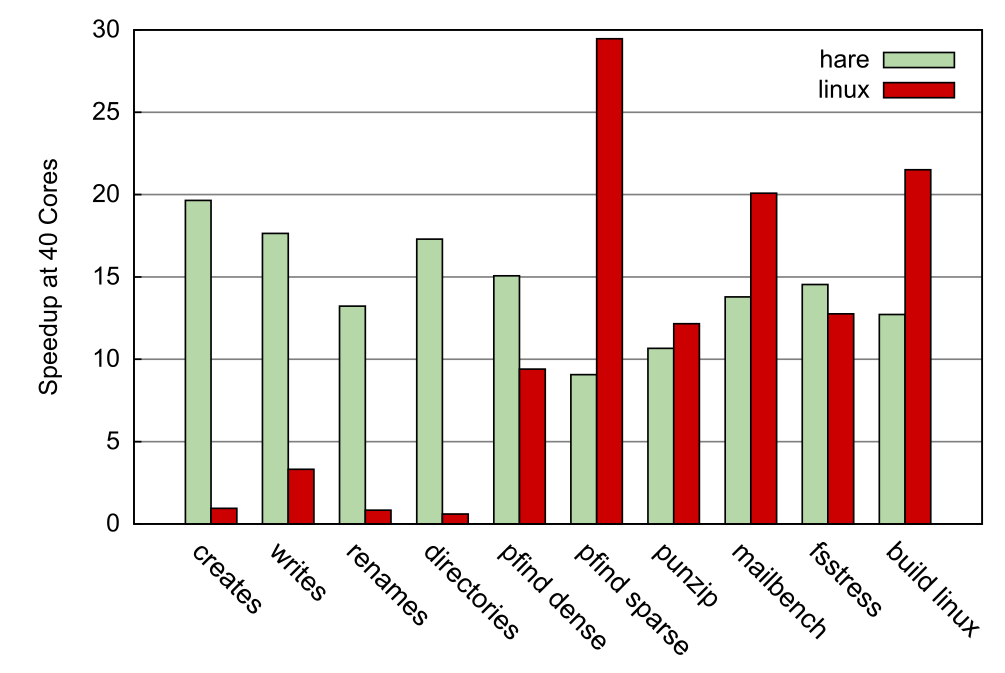
\includegraphics[scale=0.25]{hare-linux}
          \caption{Accélération de Hare comparée à Linux. On voit que Hare est
            bien plus efficace avec des microbenchmark.}
        \end{subfigure}
        \caption{Résultats des benchmark et microbenchmark exécutés sur
          Hare~\citep{gruenwald2014providing}.}
        \label{fig:hare-res}
      \end{figure}

      Dans le cas de la migration de processus, l'approche de Hare est également
      intéressante. En effet, la bibliothèque impose que la migration sur un
      autre c\oe ur soit effectuée uniquement lors d'un appel à une fonction de
      la famille \texttt{exec()}. Celle-ci a été ré-implémentée dans le noyau
      et, dans le cas d'une migration, fonctionne comme un appel de fonction via
      RPC\nomenclature{RPC}{Remote Procedure Call}. Une fois déplacé, un
      processus restera sur le même processeur jusqu'à sa libération. Pour
      assurer la cohérence des descripteurs de fichiers entre processus,
      l'initiateur du \texttt{exec()} sur le noyau source n'est pas détruit mais
      est utilisé comme \textit{proxy}. C'est à lui que s'adressera le nouveau
      processus s'il désire accéder à d'anciens descripteurs de fichiers. Le
      \textit{proxy} se charge de relayer les signaux qui sont destinés au
      processus.

      Cette approche a des avantages et des inconvénients. Un avantage certain
      est de conserver la localité des accès mémoire pour les processus ``d'une
      même famille''. Nous considérons des processus d'une même famille comme
      les processus appelant la fonction \texttt{fork()} mais jamais
      \texttt{exec()}\footnote{Notamment Firefox dont la gestion mémoire est en
        cours de changement pour ne plus utiliser un thread par onglet mais un
        processus~\citep{mozillaElectrolysis}}. En imposant la migration lors du
      \texttt{exec()}, on conserve la localité et la parenté. Néanmoins,
      l'inconvénient majeur de cette solution est sa granularité. En choisissant
      de migrer des processus entiers et non un certain nombre de threads par
      processus, et en imposant la migration uniquement lors de l'appel à
      \texttt{exec()}, Hare ne permet pas la parallélisation massive des
      applications.


    \subsection{Popcorn Linux}

      Nous allons maintenant étudier les réponses apportées
      par~\citet{katz2013popcorn} pour la migration de processus ou de thread
      dans un multi-noyau, à savoir: \benumline \item les \textit{shadow
        task} \item la définition des informations nécessaires à une
      migration \item la consistance des espaces d'adressages, virtuels comme
      physiques\eenumline.

      \begin{paragraph}{Shadow Task:}

        Popcorn Linux propose une nouvelle abstraction dans le noyau Linux :
        \textit{shadow task}. Celle-ci permet d'assurer le mécanisme de
        consistence que nous verrons par la suite.

        Lors de la migration d'un thread, la \texttt{struct task} qui le
        représente n'est pas libérée une fois la migration terminée. Le thread
        est placé à l'état \textit{sleep}, la structure est conservée en mémoire
        et placée dans une liste de \textit{shadow task}. Elle restera à l'état
        \textit{shadow} jusqu'à ce que le thread migré reviennent s'exécuter sur
        le noyau en question, ou si le processus termine son exécution. Dans ce
        cas, il envoie un message \texttt{exit()} en \textit{broadcast} à tous
        les noyaux. Les \texttt{struct task} de tous ses threads sont alors
        libérées.

        Une autre structure liée à la \texttt{struct task} est conservée: la
        \texttt{struct mm}. Celle-ci contient toutes les informations relatives
        à la mémoire physique d'un processus. La \texttt{struct mm} est
        conservée jusqu'à la réception d'un signal \texttt{exit()}. Même s'il
        n'existe plus de threads d'un processus $P$ sur un noyau $N$, la
        structure est conservée car il existe encore des instances de $P$
        ailleurs sur la machine, qui peuvent avoir besoin des informations de
        mapping qui ont été crées sur $N$.\\

        Conserver ces structures à de nombreux avantages:\benumline \item
        si la tâche revient s'exécuter sur le noyau, son redémarrage est
        beaucoup plus rapide puisque l'on s'affranchi de l'allocation
        mémoire \item cela permet de conserver les informations du thread
        concernant les pages physiques occupées \item elles permettent de
        relayer les signaux des processus entre les noyaux\eenumline.

      \end{paragraph}

      \begin{paragraph}{La migration: }
        Migrer un processus entre deux instances d'un noyau est une opération
        complexe. Il faut pouvoir re-créer un contexte d'exécution dans un autre
        espace d'adressage tout en conservant une cohérence entre les espaces
        virtuels, mais aussi physiques. Lors d'une migration de thread, il est
        nécessaire de fournir les adresses virtuelles de début et de fin:
        \begin{itemize}
          \item de la pile utilisateur
          \item du tas
          \item de l'environnement d'exécution (le code)
          \item des arguments
          \item des données
        \end{itemize}
        Ces informations permettent de maintenir la cohérence de l'espace
        virtuel du thread. Pour maintenir la cohérence de l'identification et de
        l'exécution, il faut envoyer les informations suivantes:
        \begin{itemize}
          \item le \texttt{pid}
          \item l'identifiant du noyau d'origine
          \item le \texttt{pid} sur le noyau d'origine
          \item l'identificateur de groupe
          \item la priorité
          \item la politique d'ordonnancement
        \end{itemize}
        Une fois toutes ces données reçues, le noyau de destination crée un
        thread avec les données d'identification et d'exécution adéquates, puis
        copie l'espace virtuel reçu dans celui du thread.

        \begin{figure}[ht]
          \begin{subfigure}[b]{0.45\textwidth}
            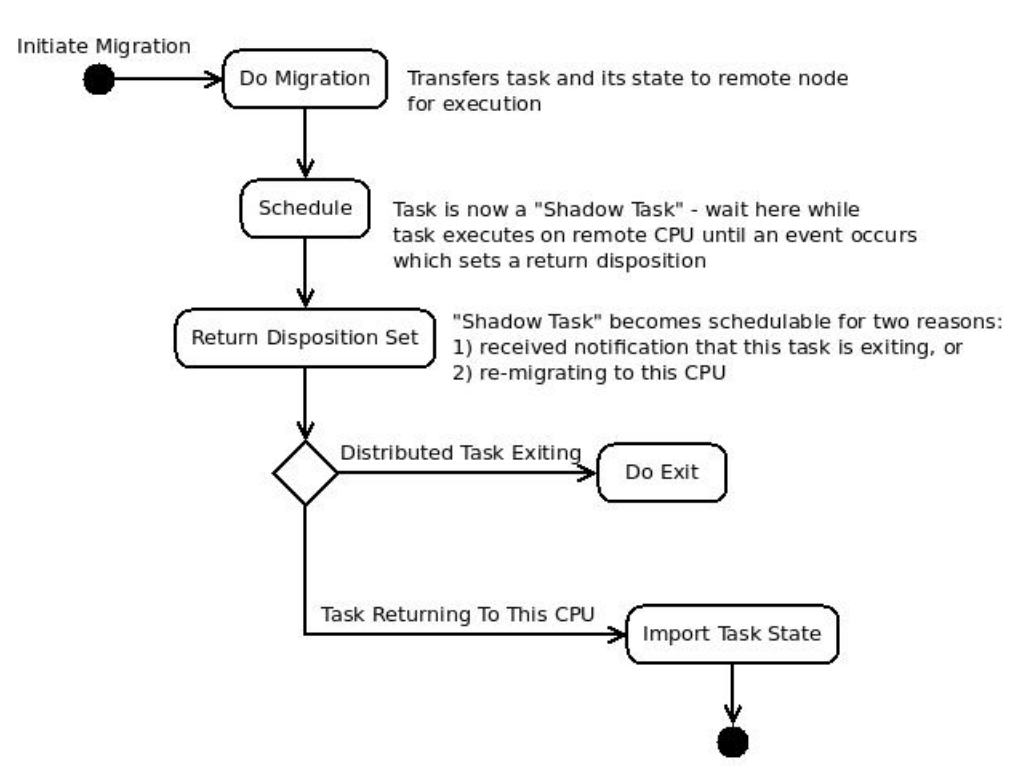
\includegraphics[scale=0.23]{popcorn-migrate-src}
            \caption{}
            \label{fig:popcorn-migrate-src}
          \end{subfigure}
          \begin{subfigure}[b]{0.5\textwidth}
            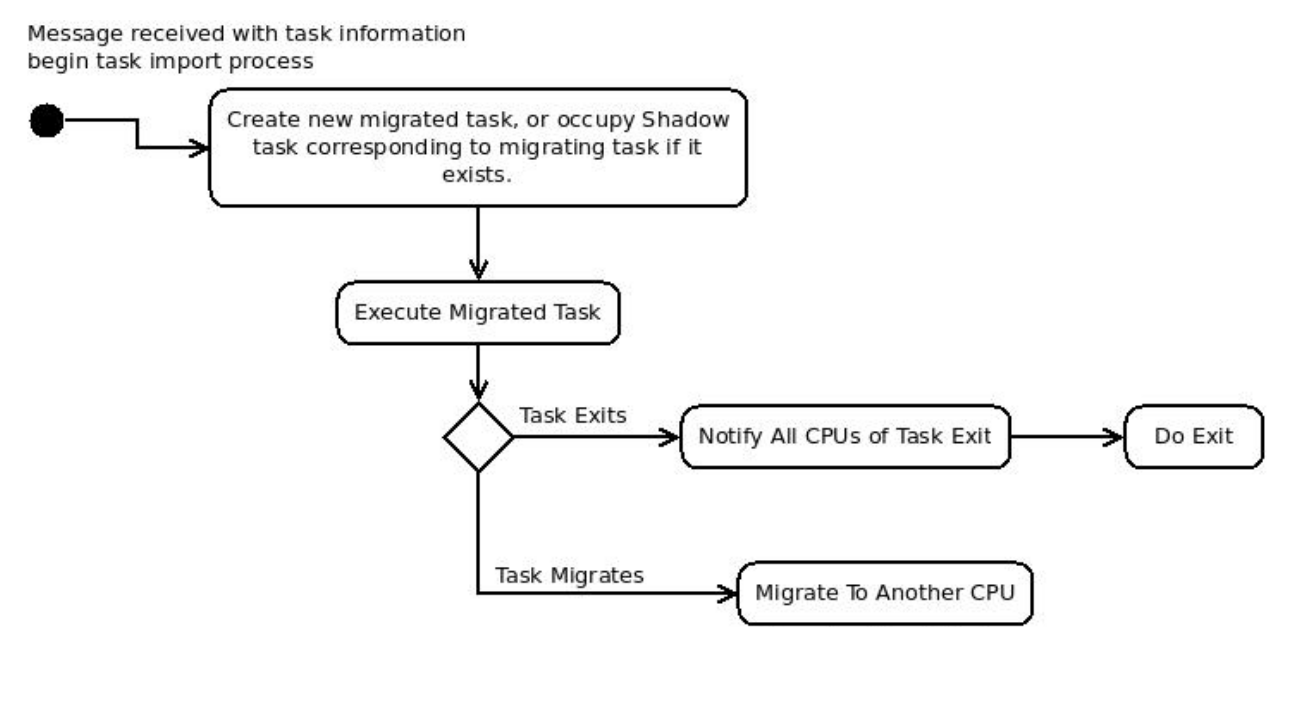
\includegraphics[scale=0.23]{popcorn-migrate-dst}
            \caption{}
            \label{fig:popcorn-migrate-dst}
          \end{subfigure}
          \caption{Actions effectuées par le noyau source (a) et destination (b)
            lors d'une migration~\citep{katz2013popcorn}.}
        \end{figure}

      \end{paragraph}

      \begin{paragraph}{Consistence des espaces d'adressage:}
        Dans sa thèse,~\citeauthor{katz2013popcorn} a identifié les propriétés
        que doit garantir une migration de processus cohérente. Les informations
        suivantes doivent être identiques sur tous les noyaux en cours
        d'exécution:
        \begin{itemize}
          \item l'espace virtuel
          \item l'espace physique\footnote{Doit être identique à 100\%, ou ne
            pas être du tout représenté}
          \item les bits de protection
          \item les pages spéciales : \textit{copy-on-write}, zero,\ldots\\
        \end{itemize}

        L'espace virtuel d'un thread est maintenu cohérent car il est
        entièrement recopié à chaque migration. En revanche, l'espace physique
        n'est pas transmis lors de celle-ci. La consistence de l'espace physique
        est gérée par la modification du gestionnaire de défaut de page de
        Linux, et par les \textit{shadow task} vues précédemment.\\

        Lorsqu'un processus veut accéder à une adresse virtuelle n'ayant pas de
        correspondance dans l'espace physique, le noyau lance une exception
        appelée \textit{page fault} ou défaut de page. Cette situation est
        possible car Linux utilise une stratégie d'allocation dite
        \textit{lazy}. Lors de la création d'un processus, il n'alloue pas
        toutes les pages physiques nécessaires mais note uniquement le fait que
        le processus aura besoin de ces pages. Elles seront réellement allouées
        lors de leur premier accès.

        Ce mécanisme est le même dans Popcorn Linux, mais une opération a été
        ajoutée avant l'allocation de la page. En effet, le noyau où le thread a
        engendré cette exception va envoyer un message en \textit{broadcast} à
        tous les autres en précisant :\benumline \item le groupe de thread
        auquel appartient l'initiateur de la faute et \item l'adresse virtuelle
        demandée\eenumline. À la réception de ce message, les noyaux vont alors
        regarder dans toutes les \textit{shadow task} qu'ils possèdent s'il n'y
        en a pas une correspondant à la requête. Si oui, alors la \texttt{struct
          mm} correspondante sera utilisée pour résoudre la mapping physique, et
        assurera ainsi la cohérence. Cette méthode, également basée sur le
        modèle \textit{lazy}, s'appelle \textit{On-Demande Address Space
          Migration}. Elle permet de réduire le coût de l'opération de
        migration, et d'avoir uniquement les pages utilisées dans les tables
        des pages des threads.

        \begin{paragraph}{Remarque:}
          Il existe de nombreux problèmes liés aux opérations concurentes en
          mémoire physique (\texttt{mmap(), mprotect(), etc\ldots}). Les
          mécanismes de cohérences présentés ici ont été simplifiés.\\
        \end{paragraph}

      \end{paragraph}

      Popcorn Linux apporte une réponse très intéressante à la problématique de
      la migration de processus ou de threads. Néanmoins, il subsiste un
      problème: la localité des accès mémoire. Ici, les threads peuvent être
      transférés entre les noyaux, mais les espaces physiques qu'ils utilisent
      sont statiques. On paye donc le coût des accès NUMA pour chaque thread
      migré en dehors de son cluster. De plus, bien qu'identifié
      par~\citeauthor{katz2013popcorn} comme étant un point critique lors d'une
      migration, Popcorn Linux n'apporte pour l'instant aucune réponse quant à
      la cohérence des descripteurs de fichiers~\citep[pageo
        4]{katz2013popcorn}. Enfin, les tests de performances (figure
      ~\ref{fig:popcorn-bench}) ont montré un surcoût non négligeable liés au
      passage de messages et à l'acquisition de verrous pour les accès
      atomiques.

      \begin{figure}[ht]
        \centering 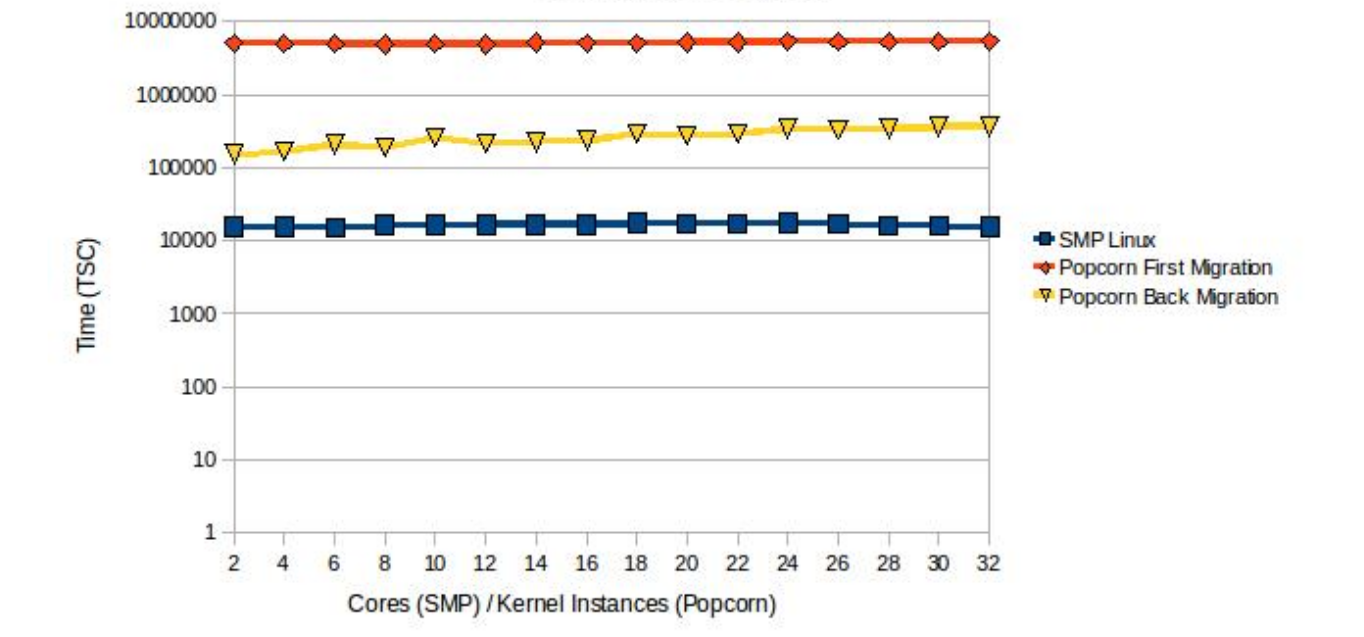
\includegraphics[scale=0.67]{popcorn-bench}
        \caption{Temps de migration d'un thread sur Linux et sur Popcorn Linux
          \itshape i) \upshape lors de la première migration \itshape ii)
          \upshape lors d'un retour sur un précédent
          noyau~\citep{katz2013popcorn}.}
        \label{fig:popcorn-bench}
      \end{figure}


      %% \subsection{DragonFly BSD}
